\chapter{Analysis of exponential integration methods in JAGUAR}

\begin{tcolorbox}[title=Résumé du chapitre : Analyse des méthodes d'intégration exponentielles dans JAGUAR, colframe=black!50!white]
  \paragraph{}
  Le but de ce chapitre est de comparer les méthodes exponentielles aux méthodes d'intégration classiques de JAGUAR pour valider leur intérêt.

  \paragraph{}
  Nous avons montré dans le chapitre précédent que CEDRE n'était pas le contexte idéal afin d'analyser des méthodes d'intégration temporelles très précises comme celles qui nous intéressent.
  Nous utilisons donc le solveur JAGUAR, basé sur la méthode des Differences Spectrales, que nous présentons au début de ce chapitre.

  \paragraph{}
  Nous analysons ensuite les méthodes exponentielles ajoutées à JAGUAR grâce à l'utilisation de la librairie SLEPc sur un cas simple, afin de constater l'ordre de ces méthodes à travers l'erreur globale en fin de simulation.
  Sur un autre cas académique, nous comparons ensuite notre ensemble de méthodes en regardant le temps d'exécution qu'il leur est nécessaire afin de réaliser une même simulation.
  Pour finir, nous utilisons les méthodes exponentielles sur un cas plus significatif car proche d'une application réelle du solveur: une aube de turbine.
\end{tcolorbox}

  \paragraph{}
  We want to analyse time exponential integration methods in a framework that gives us access to high-order spatial discretisation methods.
  It is possible to use high-order Finite Volume methods, but this means using larger stencils which hurts parallelism.
  In CEDRE, users often stop at second-order methods, so we need to use another solver.
  As the spatial discretisation method does not play a direct role in the time integration and the work done in this thesis, we can step out from the Finite Volume framework.
  Furthermore, using a less complex solver will also help us try and develop new methods more easily than we already did with CEDRE.
  This is why we decided to accomplish our analysis of exponential time integration methods with the solver JAGUAR.


  \section{JAGUAR: a Spectral Difference solver}

    \paragraph{}
    JAGUAR means proJect of an Aerodynamic solver using General Unstructured grids And high ordeR schemes.
    It is a reactive Navier--Stokes solver originally developed at CERFACS, \PS{the European center for research and advanced training in scientific computing\footnote{je vois pas l'intérêt de le mettre en anglais, soit ça soit j'enlève}}, and is jointly own by ONERA and CERFACS for four years.
    It is made for unstructured grids and uses a Large Eddy Simulation model to solve unsteady turbulence effects.
    It means that the large turbulence scales are computed explicitly while the smaller ones are modelled.
    Its particularity is that it uses a spectral method as spatial discretisation scheme: the Spectral Difference method.
    \PS{The Spectral Difference method follows some principles of the Discontinuous Galerkin formulation, in the sense that both are families of schemes of arbitrary order using polynomial approximations, but their mathematical foundations differ.}


    \subsection{The Spectral Difference method}

      \paragraph{}
      With the Spectral Difference method, the solution is represented by a polynomial of degree $p$ inside each cell.
      It means that in the partial differential equation
      \begin{equation}\label{eq:pde_2}
        \frac{\partial u}{\partial t} + \nabla \cdot F\left(u\right) = 0 ,
      \end{equation}
      $u$ is a $p$-degree polynomial of the coordinate variables, where the polynomial coefficients are functions of time.
      Then $F\left(u\right)$ has to be a $p\!+\!1$-order polynomial of the coordinate variables in order to have a $p$-order polynomial of the flux divergence.
      The key to the Spectral Difference method is how to compute a $p + 1$-order $F\left(u\right)$ from a $p$-order $u$.
      This method uses key elements that were first mentioned by \cite{Kopriva1996}, and were later developed by \cite{LiuVinokurWang2006}.

      \begin{figure}
        \centering
        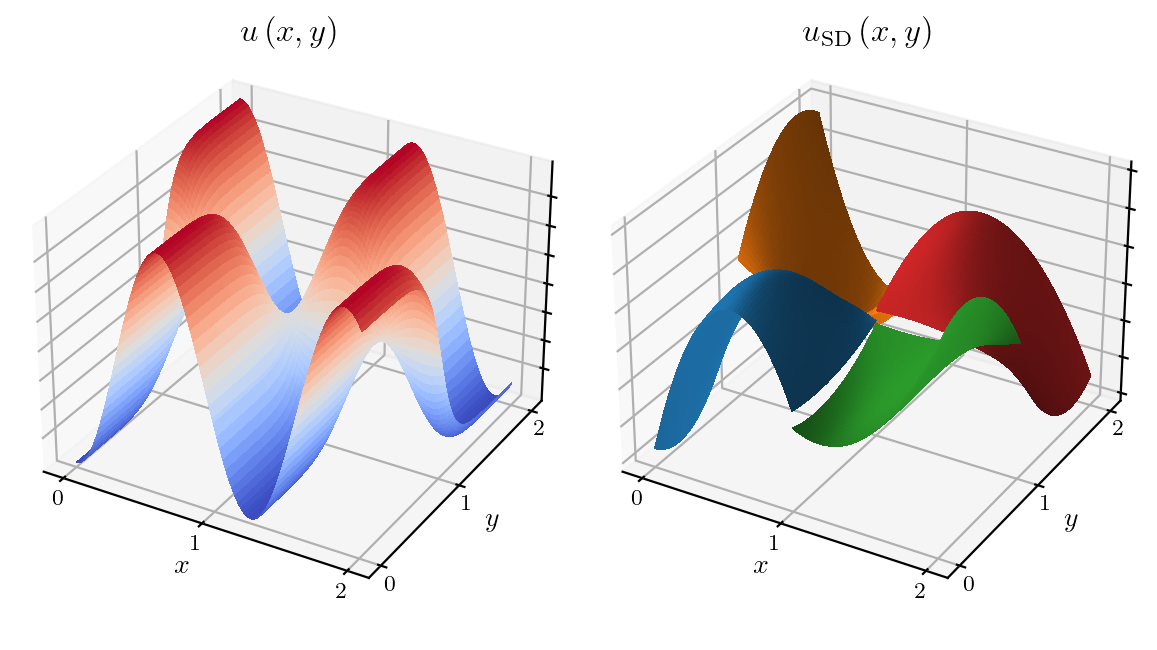
\includegraphics{figures/sd_discontinuous.png}
        \caption{Continuous function (left) and discontinuous representation made by the Spectral Difference method (right).}
        \label{fig:sd_discontinuous}
      \end{figure}

      \paragraph{}
      Because the solution is represented in each cell by a polynomial, there is no reason for the solution to be continuous throughout cell interfaces.
      Indeed, the Spectral Difference method uses a piecewise representation of the solution.
      For example, let us consider the two-dimensional regular mesh, made of $2 \times 2$ cells over $\left[0, 2\right]^2$.
      The exact analytical function $u$ over the mesh in the left part of figure \ref{fig:sd_discontinuous}:
      \begin{equation}
        \begin{aligned}
          u \colon \left[0, 2\right]^2 &\to \mathbb{R}\\
          \left(x, y\right) &\mapsto \cos\left(5x\right) \tanh\left(5\left(1 - y\right)\right)
        \end{aligned}
      \end{equation}
      cannot be represented by polynomial exactly and the right picture of figure \ref{fig:sd_discontinuous} represents the solution associated with the Spectral Difference method.
      The colour mapping corresponds to the output of the function but is not given as this function is of no particular interest: it is a rough example only.
      This function is interpolated with a second-order method using Lagrange polynomials over each cell.
      The result is shown in the right part of figure \ref{fig:sd_discontinuous}, where each colour corresponds to one cell.
      There are discontinuities at the cell interfaces, which shows a specificity of the Spectral Difference methods.
      If the function on the left part of figure \ref{fig:sd_discontinuous} was used as an initial condition for a simulation, the Spectral Difference method would in fact use the polynomial interpolation on the right part.
      However, to respect the underlying conservation property of equation (\ref{eq:pde_2}), it is necessary for $F$ to be continuous over the whole computational domain.
      The Spectral Difference method will then make sure that the polynomial representations of the flux density are continuous throughout cell interfaces.

      \paragraph{}
      To better understand how this method works, let us take a one-dimensional cell: the segment $\left[0, 1\right]$.
      Because the following is done at a fixed time, the dependency on the time is dropped, but the solution and the coefficients are in reality functions of the time, not scalars.
      The solution $u$ inside this segment is then $u\left(x\right) = \sum_{i=0}^p a_ix^i$.
      Using Lagrange interpolation polynomials, it is equivalent to use the set of the $p + 1$ coefficients $a_i$ or the set of the $p + 1$ values $u\left(x_i\right)$ computed at the distinct points $x_i \in \left[0, 1\right]$ called \emph{solution points}.
      The solution as a $p$-order polynomial is represented by either one of those two sets.
      As the flux density $F$ must be a $p\!+\!1$-order polynomial, it can also be represented by its values in the $p + 2$ distinct \emph{flux points}.
      To ensure that $F$ is continuous at the segment end points, we take $0$ and $1$ as flux points.
      The choice of the rest of the flux points will be discussed later, but let us say for now that they are staggered with the solution points: each flux point, apart from the segment end points, is between two solution points and vice versa.

      \begin{figure}
        \centering
        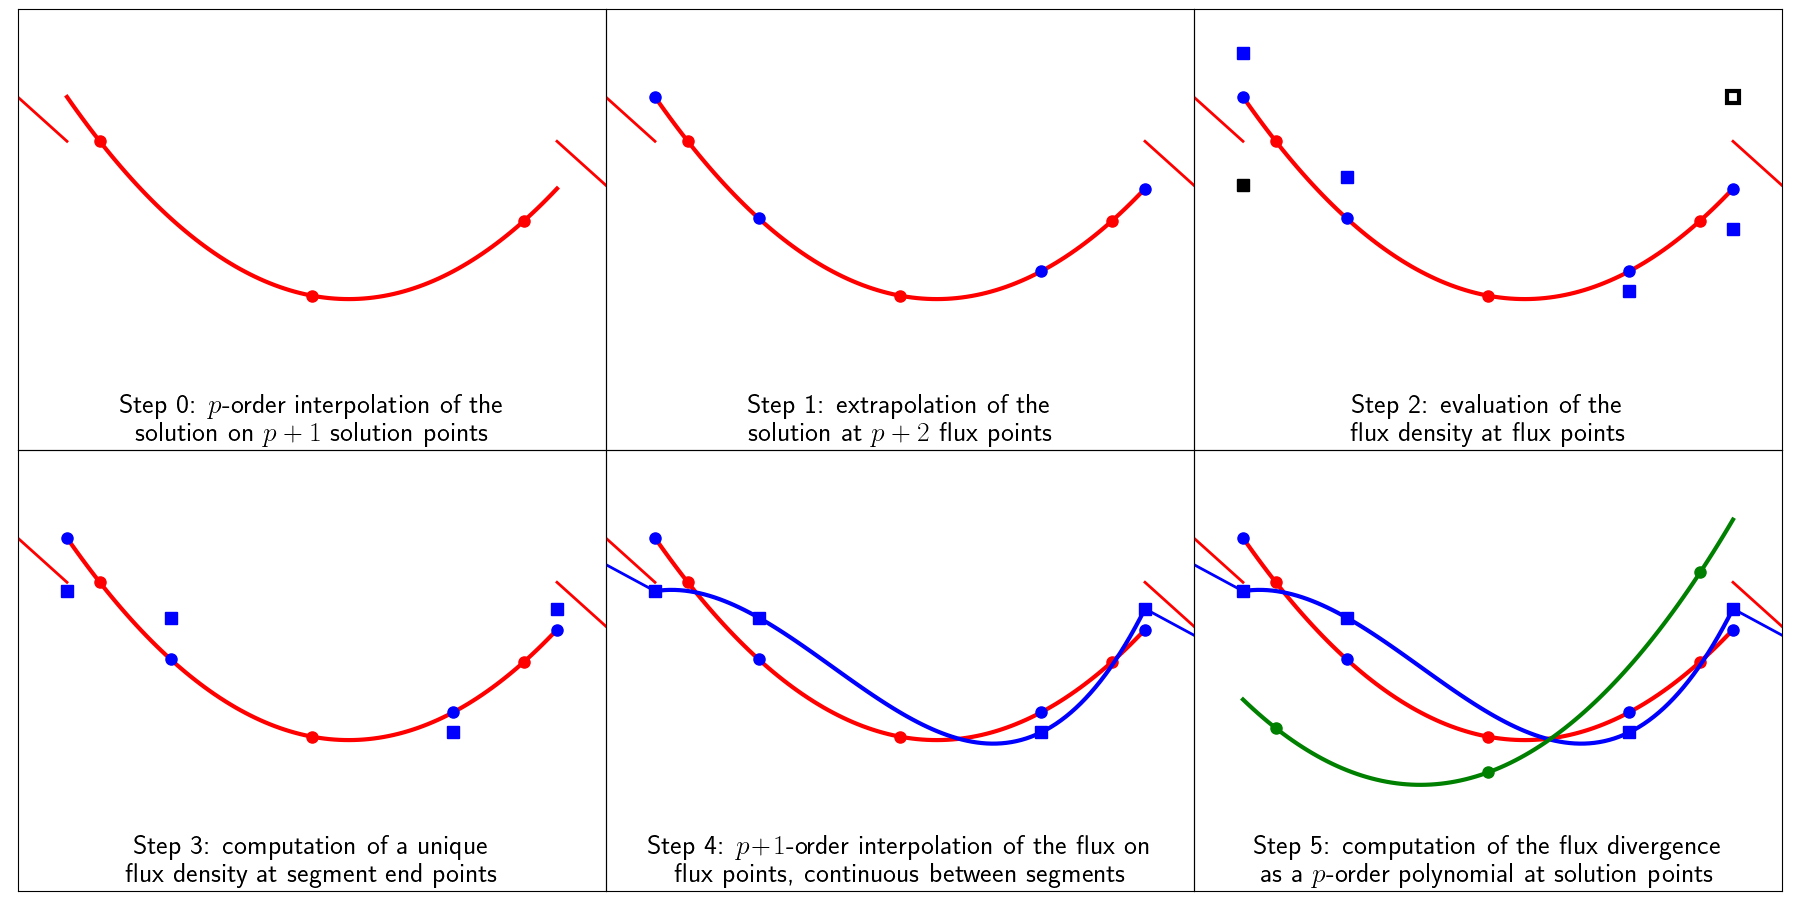
\includegraphics{figures/sd_scheme.png}
        \caption{Steps of the Spectral Difference methods with $p = 2$.}
        \label{fig:sd_scheme}
      \end{figure}

      \paragraph{}
      Figure \ref{fig:sd_scheme} shows the steps the Spectral Difference make to compute the flux divergence $\nabla \cdot F\left(u\right)$ from the solution $u$, with the specific choice $p = 2$.
      \begin{enumerate}
        \setcounter{enumi}{-1}
        \item At first, the solution is represented with a red line by its value in the $p + 1$ solution points.
        The solution points are marked by red dots.
        Parts of the solution from the left and right neighbouring cells can be seen.
        As the figure shows, the piecewise local solutions inside each cell may be discontinuous at the mesh interface.
        This is the starting point of the Spectral Difference method and will be called the 0-th step.
        \item In the first step, the method computes the value of the solution in the $p + 2$ flux points, marked by blue dots.
        As the polynomial representing the solution is known, this step just consists in evaluating it at flux points.
        \item In the second step, the method evaluates the flux density $F\left(u\right)$ in each flux point.
        This is possible because the solution was computed in those points in the previous step.
        The values of the flux density are marked by blue squares in the figure.
        However, segment end points are flux points for the two neighbouring cells, and therefore the figure shows a full black square for the flux at $0$ from the left neighbouring cell and an empty black square for the flux at $1$ from the right neighbouring cell to highlight this discontinuity.
        \item Because there are different values of the flux density at the segment end points, the method would not preserve the conservative property of the partial differential equation.
        This is why in the third step, the method computes a unique interface flux density for both cells at each segment end points.
        The problem is to find the interface flux at the discontinuity of a piecewise solution.
        In other words, this is a Riemann problem.
        Once again, this is solved with a Riemann solver, exact or approximate, to get in the end a single value for the left and right parts of the discontinuity.
        \item An interpolation from the value of the flux density at the $p+2$ flux points using Lagrange polynomials enables to get a $p+1$ order $F$ as expected in the fourth step, represented with a blue line in the figure.
        Therefore, one can end up with a continuous representation of $F$, differentiable everywhere except at cell interfaces.
        \item In the last step, the representation of $F$ is differentiated to get the flux divergence, represented by a green line in the figure.
        Finally, a time integration method can use a $p$-order representation of $\nabla \cdot F$ to compute the solution at the next time step.
      \end{enumerate}

      \paragraph{}
      To work with any segment, not only $\left[0, 1\right]$, an isoparametric transformation is introduced to get back to this unity segment.
      It is the same when working with multiple dimensions, where the isoparametric transformation gets the cell back to the tensor powers of this segment.
      The placement of the solution points does not seem to matter much, but the placement of the flux points does \cite{VandenAbeeleLacorWang2008}.
      The $p + 1$ solution points we will use are defined in the $\left[0, 1\right]$ segment as the Chebyshev roots:
      \begin{equation}
        x_i = \frac{1}{2} \left(1 - \cos\left(\frac{2i + 1}{2p + 2} \pi\right)\right), \quad 0 \leq i \leq p .
      \end{equation}
      They are traditionally defined inside the $\left[-1, 1\right]$ segment but are scaled into $\left[0, 1\right]$.
      They are the roots of the Chebyshev polynomials of the first kind and are often used in polynomial interpolation as they tend to minimise Runge's phenomenon.
      The $p + 2$ flux points are the $p$ roots of the $p$-th Legendre polynomials to which are added the two segment end points.
      This choice has the property that there is a flux point between each contiguous solution point.
      There is no explicit formula for the Legendre polynomial roots as there is one for the Chebyshev polynomial roots.
      They are also defined in the $\left[-1, 1\right]$ segment and are scaled into $\left[0, 1\right]$.
      Finally, the solution and flux points can be seen in figure \ref{fig:sd_points}.

      \begin{figure}
        \centering
        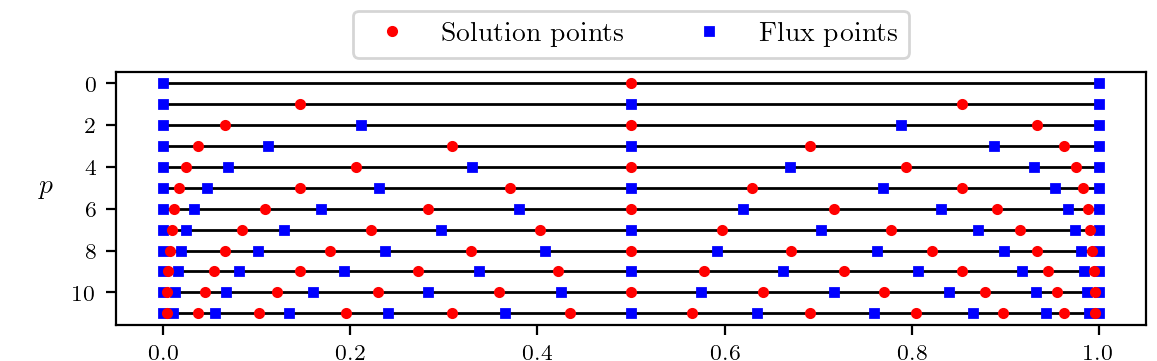
\includegraphics{figures/sd_points.png}
        \caption{Solution points and flux points in the $\left[0, 1\right]$ segment used in the Spectral Difference method for $0 \leq p \leq 11$.}
        \label{fig:sd_points}
      \end{figure}

      \paragraph{}
      As a side note, the Spectral Difference method with $p = 0$ corresponds roughly\footnote{\PS{Pourquoi roughly?}} to the first-order Finite Volume method.
      Indeed, the solution is assumed constant in the cell, represented by the value at its barycenter.
      The flux balance is made at the cell interfaces with a Riemann solver.
      This corresponds to the placement of the solution and flux points in figure \ref{fig:sd_points} when $p = 0$.
      For higher $p$, the proposed Spectral Difference method is naturally of order $p$
      Indeed, the method can represent exactly any polynomial of degree $p\!-\!1$ and, as a consequence, the error term is of order $p$.
      In JAGUAR, the order $p$ range from 2 to 10, but $2 \le p \le 6$ for practical applications.

      \paragraph{}
      The demonstration of the accuracy of the Spectral Difference method is proposed in a reference paper published recently \cite{VanharenPuigtVasseurEtAl2017}.
      JAGUAR was optimised to be efficient for parallel computations \cite{Cassagne2014, CassagnePuigtBoussuge2015, Marait2015}.
      To perform Large Eddy Simulation, it is of paramount importance to implement unsteady characteristic boundary condition: Navier--Stokes Characteristic Boundary Condition, or NSCBC.
      The initial formulation \cite{FievetDeniauPiot2020} was extended to deal with acoustic conditions and liner optimisation \cite{CardesaFievetPiotEtAl2022}.
      Recently, the solver was extended to handle $h-p$ adaptation \cite{HartmannBalanBassiEtAl2021} and the schemes were extended to triangles and tetrahedrons \cite{VeilleuxPuigtDeniauEtAl2022, VeilleuxPuigtDeniauEtAl2022a}.
      Another improvement concerns the treatment of combustion, with a PhD thesis funded by Safran \cite{MarchalDeniauBoussugeEtAl2021}.
      Finally, the last extension concerns the treatment of shocks \cite{DeniauPuigt2022}.
      This review shows the strong involvement of researchers on the solver.


    \subsection{Exponential integration methods in JAGUAR}

      \paragraph{}
      Using a high-order spatial discretisation method and a refined mesh is the best suited situation to test high-order time integration methods: the resulting error will come mostly from the time integration and not the spatial discretisation.
      The development of an exponential time integration method was inexpensive within CEDRE as the method reuses lots of already existing parts.
      For JAGUAR which only has explicit methods, the Arnoldi iteration and the exponential computation functions must be implemented to use exponential methods.
      They could be developed as internal stand-alone routines to produce a finely tuned method for JAGUAR.
      However, since the goal is to analyse exponential methods scientifically, it was decided to rely on the SLEPc library \cite{HernandezRomanVidal2005}.
      The Scalable Library for Eigenvalue Problem Computation, or SLEPc, is an extension of the software library PETSc \cite{petsc-web-page, petsc-user-ref, petsc-efficient}.
      Instead of rewriting the needed algorithms, it was chosen to use their SLEPc implementation.
      In particular, SLEPc handles what it calls \emph{Matrix Function} objects or MFN:
      \begin{quote}
        "Given a matrix $A$ and a vector $b$, the call \mintinline{c}{MFNSolve(mfn, b, x)} computes \\
        $x=f\left(A\right) b$, where $f$ is a function such as the exponential."
      \end{quote}
      This is precisely what is needed to develop exponential methods: as it handles the previously introduced $\varphi$-functions with its MFN objects, SLEPc is then an obvious choice of a library for implementing exponential integration methods.
      Furthermore, because it relies on PETSc, it is efficiently scalable to fit our multiprocessing needs.

      \paragraph{}
      Exponential methods are based on a decomposition of the ordinary differential equation such as equation (\ref{eq:ode_split}).
      However, JAGUAR uses only explicit time integration methods, so no Jacobian matrix is available.
      Computing analytically the Jacobian matrix would prove challenging as any ingredient should be differentiated, such as the Spectral Difference scheme, the Riemann solvers, the diffusion scheme, etc.
      It is not insurmountable but would amount to more work than what could be afforded during this thesis.
      It was decided instead to reuse the work from the previous part: the Jacobian matrix will not be formed, but its effect will be computed by a finite difference approximation.
      Another reason to work with the SLEPc library is that using a finite difference approximation is easy with it.
      More precisely, it is PETSc that handles this approximation.
      \PS{To sum up, to compute $\varphi_k\left(L\right)b$ that is required for the exponential methods with $L = f'\left(y\right)$, $L$ is created with the appropriate PETSc data type.
      As it is a Jacobian matrix of a function, PETSc only needs to know the function to compute matrix-vector products.}
      Then, after setting the MFN object of SLEPc, the library can compute the desired result
      The Arnoldi iteration, the Scaling and Squaring algorithm and the exponential evaluation are all handled internally by the library.
      Overall, this procedure is extremely simple from our perspective and requires only a few lines of code to implement.
      This highlights the relevance of using the SLEPc library to easily test procedures and acquire the associated knowledge.

      \paragraph{}
      Other people that also work with JAGUAR did develop implicit time integration methods using PETSc.
      To continue in this direction, it was decided to add a time integration method based on the generic PETSc Time Stepper \cite{AbhyankarBrownConstantinescuEtAl2018}.
      This way, a user may use most methods from PETSc in JAGUAR with no additional developments.
      It includes any explicit and implicit time integration methods, but also nonlinear solvers such as Newton's methods with various line search algorithms, linear solvers with various Krylov subspace methods and finally various preconditioning.
      However, this generic PETSc Time Stepper method was added on the side of this thesis, and therefore will not be discussed here, along with the previous work on implicit methods.


    \paragraph{}
    In the end, the high-order spatial discretisation method called the Spectral Difference method allows to analyse and compare exponential methods that are available through the SLEPc library.
    In the following, attention is mainly focused on the three methods that were presented earlier in table \ref{tab:exprb_butcher}: the Rosenbrock--Euler, ExpRB32 and ExpRB42 methods.


  \section{Analysis of exponential time integration methods}

    \paragraph{}
    There are in JAGUAR all the tools necessary to analyse exponential time integration methods and several test case must be chosen.
    During the analysis, the exponential methods and explicit Runge--Kutta methods will be compared, as the latest ones are the only available methods in JAGUAR and represent the state-of-the-art.
    Those methods are:
    \begin{itemize}
      \item RK2, the Midpoint method
      \item RK4, the classical four-stage fourth-order method
      \item RKo6s, a low-storage, low-dissipation and low-dispersion six-stage second-order method from \cite{BogeyBailly2004} dedicated to unsteady computations
      \item TVDRK(3, 3), a three-stage third-order TVD method from \cite{ShuOsher1988, GottliebShu1996}
      \item SSPRK(5, 4), an optimal SSP five-stage fourth-order method from \cite{SpiteriRuuth2002}.
    \end{itemize}
    Low-storage methods are Runge--Kutta methods for which the matrix $A$ in their Butcher tableau is lower diagonal, or in other words all $a_{ij}$ are null except when $j = i - 1$.
    Also, all $b_i$ are null except the last one that is equal to $1$.
    It means that the final stage and all intermediate ones use only the previous stage.
    Therefore, there is no need to keep track of intermediate stages in memory, only to update the current value, which gives the name low-storage method.
    The last two methods are Runge--Kutta methods with an additional property originally called TVD \cite{GottliebShu1996} and more recently SSP  \cite{GottliebShuTadmor2001}.
    Without going into too much detail, it means that they are methods that are convex combinations of explicit Euler steps so that their stability is guaranteed for sufficiently small time steps.
    To us, it means they are defined differently than other methods, using the coefficients $\alpha_{0 < i \leq k, 0\leq j < i}$ and $\beta_{0 < i \leq k, 0\leq j < i}$ as:
    \begin{equation}
      \left\{\begin{aligned}
        y_{n+1} &= y^{\left(k\right)} \\
        \textrm{with}\quad y^{\left(i\right)} &= \sum_{j = 0}^{i-1} \alpha_{ij} y^{\left(j\right)} + \Delta t \beta_{ij} f\left(y^{\left(j\right)}\right) , \quad 1 \leq i \leq k\\
        \textrm{and}\quad y^{\left(0\right)} &= y_n
      \end{aligned}\right. .
    \end{equation}
    However, they are equivalent to traditional Runge--Kutta methods in the sense that they can be represented by the standard Butcher tableau, with:
    \begin{equation}
      \left\{\begin{aligned}
        a_{ij} &= \sum_{l = j+1}^{i-1} \alpha_{i-1, l-1} a_{l, j} + \beta_{i-1, j-1} \\
        b_i &= \sum_{l = i+1}^{k} \alpha_{k, l-1} a_{l, i} + \beta_{k, i-1}
      \end{aligned}\right. .
    \end{equation}
    We can finally say that we are indeed working with explicit Runge--Kutta methods, as they were introduced initially.


    \subsection{Order analysis: convected inviscid isentropic vortex}

      \paragraph{}
      This first case is designed to analyse the order of accuracy of the proposed methods and to validate their implementation.
      Is is the simple case of the two-dimensional inviscid isentropic vortex, the same as the one considered with CEDRE.
      The case is still described by equation \ref{eq:covo}, but the numerical values are different.
      The convective flow Mach number is still $0.5$, but this time $P_\infty = 10^5\si{\pascal}$ and $T_\infty = 300\si{\kelvin}$.
      The heat capacity ratio is $\gamma = 1.4$ and the specific gas constant is $r_\textrm{gas} = 287.058\si{\joule\per\kilo\gram\per\kelvin}$.
      Those values correspond to standard values for dry air.
      The mesh represent the two-dimensional box $\left[0, L\right]^2$ with $L = 0.1\si{\meter}$, and is made of $N \times N$ cells.
      The vortex is defined by its characteristic radius $R_0 = 0.005\si{\meter}$ and its intensity $\beta = 0.2$.
      It corresponds in fact to the same vortex as the one used with CEDRE, in size and in intensity, but it has been scaled down into a smaller box and dimensioned to some given pressure and temperature.
      The present choice is in agreement with the prescription of the International Workshop on High Order CFD Methods.

      \paragraph{}
      \GP{Quel solveur de Riemann ???? Tu ne l'as pas dit...}
      \PS{Comment ça ?}

      \paragraph{}
      The period for those numerical values is $L / U_\infty = \num{0.0005759974000734113}\si{\second}$.
      After 20 periods, the vortex should recover the initial position and the 2-norm of the error between initial and computed solutions can be defined for any scalar variable $u\left(\vec{x}, t\right)$:
      \begin{equation}
        \operatorname{err}\left(u\right) = \left(\int_{\left[0, L\right]^2} \left(u\left(\vec{x}, 20T\right) - u\left(\vec{x}, 0\right)\right)^2 \mathrm{d}\vec{x} \right)^{1/2} .
      \end{equation}
      \PS{
      %\GP{ Je vire ca car c'est pas tout à fait vrai... Because it is a periodic case, the initial value corresponds to the exact solution.
      %This error corresponds then to the error of the time integration method.}\\
      %Je mets ça à la place:
      Once the vortex moves in the domain, the numerical solution is subject to two schemes and errors are a consequence of both.
      Once the spatial scheme is defined, the mesh is chosen sufficiently refined in order to transport the vortex accurately and the goal is to have a much lower influence of the spatial scheme than of the time integration scheme on the total error.
      The order of our time integration methods can be determined by looking at this error as a function of the time step.
      }

      \paragraph{}
      The error at the end of the simulation is the global truncation error: the error the method makes while getting to a fixed time, no matter how many iterations it took.
      However, the order of a time integration method was previously defined using the local truncation error: the error it makes after a single small step.
      There is a link between global and local truncation errors for our single-step methods.
      Let us call $\tau_n$ the local truncation error and $e_n$ the global truncation error at step $n$.
      Because single-step methods can be written as:
      \begin{equation}
        y_{n+1} = y_n + \Delta t_n g\left(y_n, \Delta t_n\right) ,
      \end{equation}
      with an increment function $g$ that is $K$-Lipschitz continuous in the $y$ variable, the global truncation error is bounded \cite{SueliMayers2003}:
      \begin{equation}
        \left| e_n \right| \leq \frac{\max_{1 \leq i \leq n} \left| \tau_i \right|}{K \Delta t_n} \left(e^{K\left(t_n - t_0\right)} - 1\right) .
      \end{equation}
      A method is a $p$-order method if $\tau_n = O\left(\Delta t^{p+1}\right)$.
      Therefore, a $p$-order method verify $e_n = O\left(\Delta t^{p}\right)$.
      However, the reciprocal is not true: observing a global truncation error $e_n = O\left(\Delta t^{p}\right)$ does not mean the order of the method is $p$.
      As a consequence, attention is focused on the expected order for the global truncation error at the end of the computation, as it is the error users look at.
      The proof of the order for a method is analytical, by writing the partial Taylor series of the exact solution, as we did earlier for the exponential Rosenbrock--Euler method.

      \paragraph{}
      The point of this analysis is to see how the global truncation error depends on the time step $\Delta t$ that is kept constant throughout the computations.
      Because some methods are more accurate than others, several computations with different mesh resolutions and Spectral Difference method orders were made.
      Let us start with the Midpoint method, associated with the order of the spatial discretisation method $p = 4$. The computation is stopped after 20 periods and the $L_2$ error for the pressure is analysed for different time steps.
      Results are shown using the CFL number as it is proportional to the time step:
      \begin{equation}
        \mathcal{N}_\textrm{CFL} = \frac{N \left(p + 1\right) \left(1 + \operatorname{Ma}\right) \sqrt{\gamma r_\textrm{gas} T}}{L} \Delta t .
      \end{equation}
      Using the CFL number instead of the time step allows to compare results with different $N$ or even $p$.
      It can be seen here as a nondimensional time.
      Computations are made for multiple values of $N$: 16, 32 and 64, and the corresponding results are shown in figure \ref{fig:covo_rk2}.
      The $16\times16$ mesh does not allow for a good analysis: the error due to the spatial discretisation method is too important and prevents to see the expected dependency between the global truncation error and the time step.
      The two other meshes however show the expected relation: $\operatorname{err} = O\left(\Delta t^2\right)$.

      \begin{figure}
        \centering
        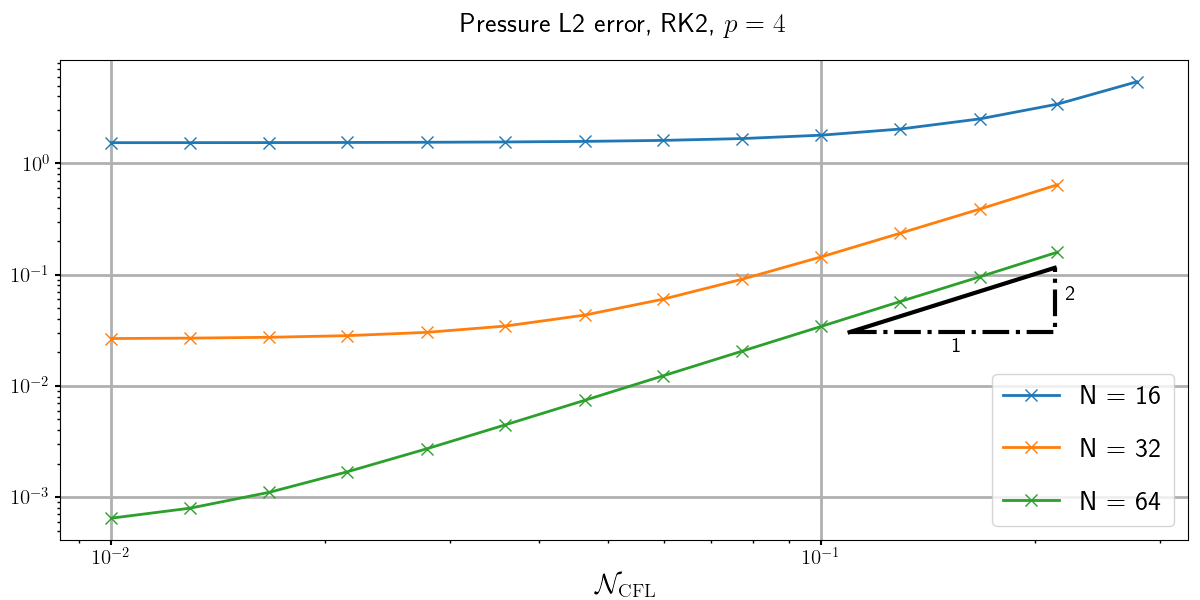
\includegraphics{figures/covo_rk2.png}
        \caption{Global truncation error for the RK2 Midpoint method.}
        \label{fig:covo_rk2}
      \end{figure}

      \paragraph{}
      This analysis is repeated for other methods, and we look now at the RK4 method.
      However, figure \ref{fig:covo_rk2_rk4} shows that the error is constant no matter the value of $N$.
      It is because the error due to the RK4 method is so small that it is dominated by the error due to the spatial discretisation scheme.
      It is useless to do the same for lower time steps, as the error would not change, therefore the RK4 error lines are continued by black dashed lines.
      As the time step decreases, the curves from the Midpoint scheme tend to the same dashed lines: this is the proof that this lower bound for the error corresponds to the error of the spatial discretisation method.
      It shows once again that a spatial discretisation method with small errors is necessary in order to analyse time integration methods.

      \begin{figure}
        \centering
        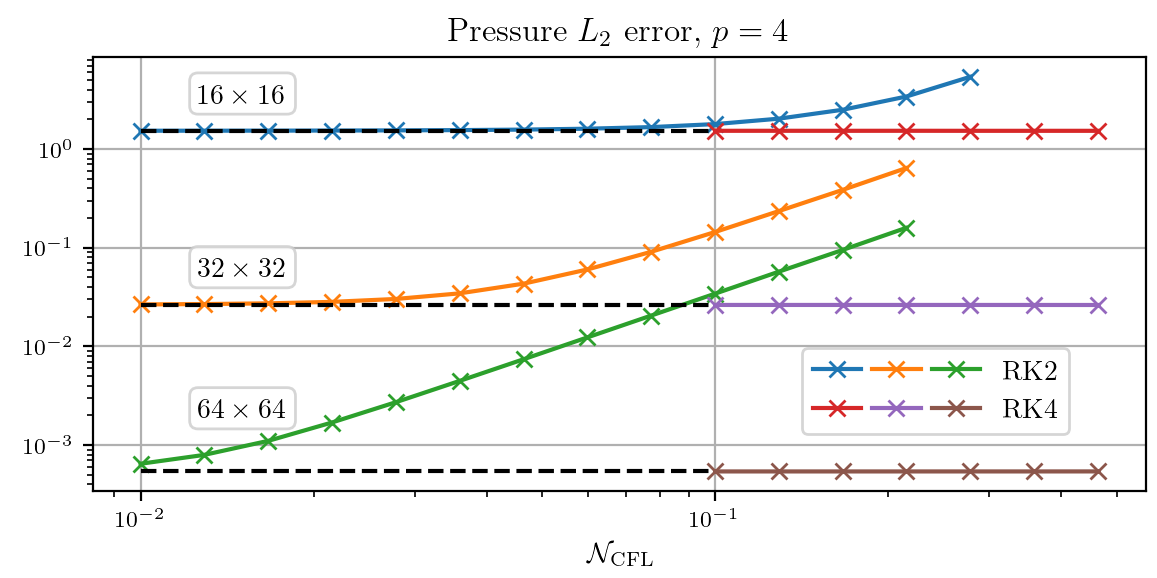
\includegraphics{figures/covo_rk2_rk4.png}
        \caption{Global truncation error for the RK2 and RK4 method.}
        \label{fig:covo_rk2_rk4}
      \end{figure}

      \paragraph{}
      Increasing $N$ up to 128 and then 256 was unsuccessful: the error was still constant.
      Instead of refining the mesh, an analysis playing with the Spectral Difference method can be performed by increasing the spatial discretisation order.
      As the theory behind this analysis does not directly depend on $N$ and $p$, we can adjust them to better fit the method we want to analyse.
      This is done in figure \ref{fig:covo_rk} where the global truncation error is shown as a function of the time step, or CFL number, for the RK4, RKo6s and TVDRK(3, 3) methods.
      The expected slopes for the second and third-order methods are obtained but the result is more subtle for the fourth-order method.
      The error is once again dominated by the error of the spatial discretisation scheme.
      On the right part of the curve, one can guess the correct slope but it is necessary to plot the error for larger time step values
      to see it more clearly.
      However, those larger time step values are outside the stability domain of the method.
      In fact, all curves end on the right at the largest time step for which the computation did not fail.
      It means from figure \ref{fig:covo_rk} that the RKo6s method is more stable than both the RK4 and TVDRK(3, 3) methods.
      This is the issue with this analysis: for too small time steps, the error from the spatial discretisation method is dominant and the expected slope are not recovered.
      On the other hand, with too large time steps, computations fall outside the stability region of the method.
      The difficulty is to find the correct window that allows to observe the desired slope by choosing suitable values for $p$ and $N$.
      Because the error of the SSPRK(5, 4) is particularly small, it was not possible to find reasonable values below $p = 8$ and $N = 64$.
      Above those values, the computations get rather long so we skipped this method.

      \begin{figure}
        \centering
        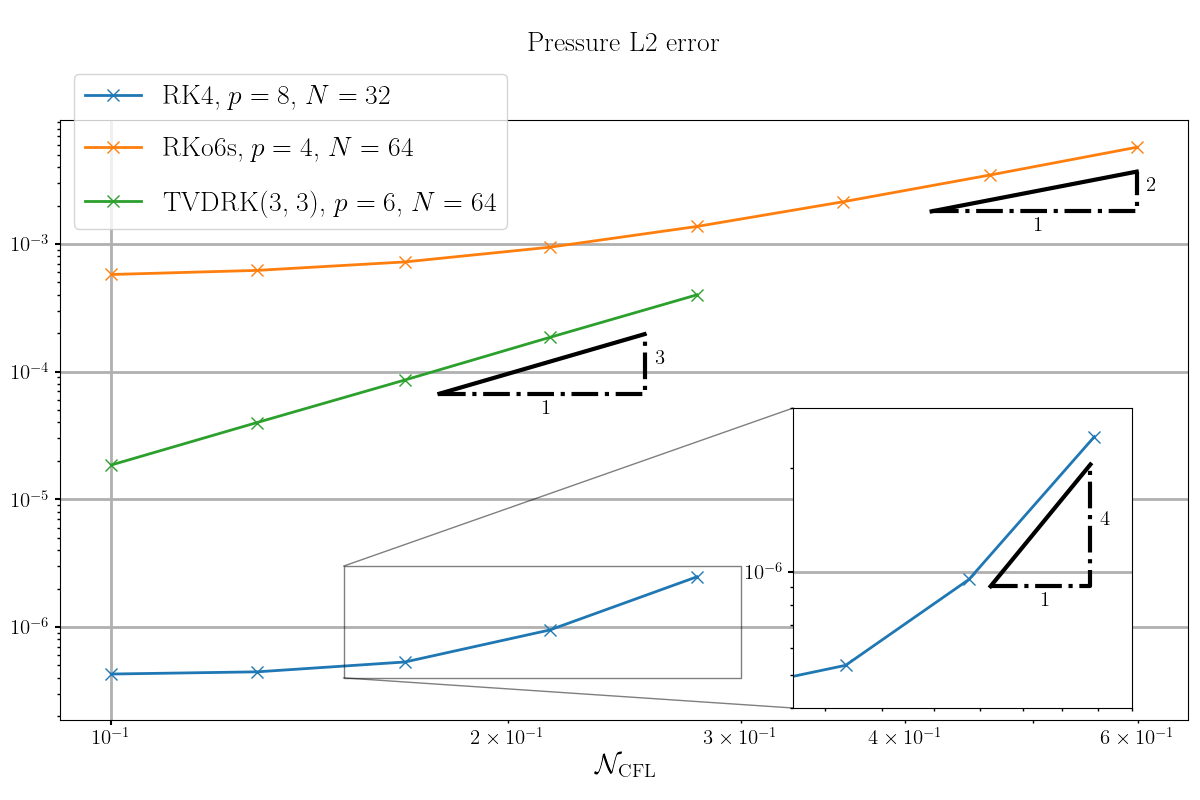
\includegraphics{figures/covo_rk.png}
        \caption{Global truncation error for the RK4, RKo6s and TVDRK(3, 3) methods.}
        \label{fig:covo_rk}
      \end{figure}

      \paragraph{}
      The analysis on traditional explicit Runge--Kutta methods can now be applied to the newly added exponential Rosenbrock methods.
      Their corresponding error curves are shown in figure \ref{fig:covo_exp}.
      As expected, the respective slope values are 2, 3 and 4.
      Furthermore, by looking at the abscissa ranges, they work correctly with higher CFL numbers than all the explicit methods that were tested.
      The goal of this first analysis of the exponential integration methods is not to analyse their robustness, but it already seems better than with explicit methods.
      What is interesting from this analysis is that one can use higher-order methods with fewer Runge--Kutta stages.
      Furthermore, the additional computational cost of the additional stages is low.
      As discussed earlier, exponential Rosenbrock methods can be reformulated as in equation (\ref{eq:exprb_defect}) using the defects $D_{n, i}$.
      The first stage of an exponential Rosenbrock method is then an exponential Rosenbrock--Euler method, for which the contribution of the "full" right-hand side $f\left(y_n\right)$ is used.
      Here, this is done with the algorithms previously described, using a Krylov subspace of dimension 20.
      Then, because the defects are relatively smaller, the other stages compute their contribution with only 5 Krylov basis vectors.
      The two exponential Rosenbrock methods with two stages are not a lot more expensive than the Rosenbrock--Euler method.
      In comparison, a 2-stage explicit Runge--Kutta method will be twice as computationally expensive as the Euler method.
      This analysis was also performed with larger Krylov subspace methods.
      In this other configuration, the first stage uses 40 Krylov basis vectors for all three exponential methods, and the second stage uses 10 Krylov basis vectors for the ExpRB32 and ExpRB42 methods.
      However, using a larger subspace did not have any impact on the result of this analysis.
      For all $\left(N, p\right)$ configurations, the error curve as a function of the time step was almost the same as with smaller Krylov subspace, such as they were almost indistinguishable when plotted in figures like figure \ref{fig:covo_exp}.

      \begin{figure}
        \centering
        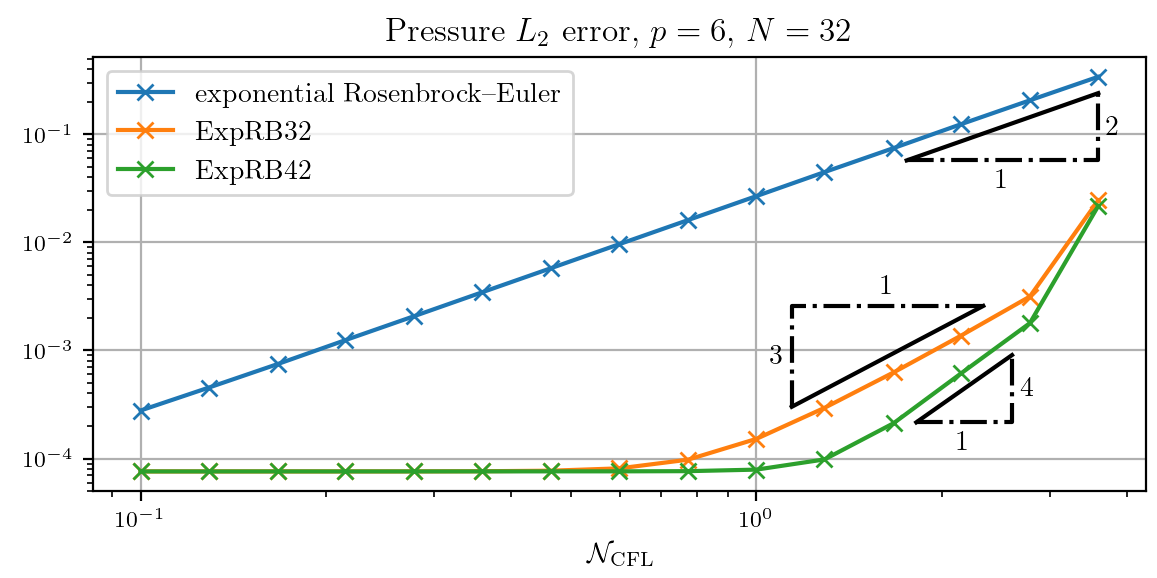
\includegraphics{figures/covo_exp.png}
        \caption{Global truncation error for the exponential Rosenbrock--Euler, ExpRB32 and ExpRB42 methods.}
        \label{fig:covo_exp}
      \end{figure}

      \paragraph{}
      We choose this first test case as it is widespread in the computational fluid dynamic community, as a tool to analyse the order of integration schemes.
      It often concerns spatial discretisation methods, but it can be considered for time integration method as it gives access to the global truncation error, which is the error that interests the solver users.
      First, this analysis recovers the correct slope on the error curve as a function of the time step for the already existing explicit Runge--Kutta integration methods.
      Indeed, the error converges, as the time step decreases, to a minimum error value that comes from the spatial discretisation scheme.
      By refining the mesh and using higher-order spatial discretisation methods, we are able to reduce this minimal error and observe the expected curve for almost all methods.
      The same analysis but with the newly implemented exponential Rosenbrock methods showed the expected order.
      It also showed that the additional cost of using more stages with exponential methods is relatively small compared to the same additional cost for explicit Runge--Kutta methods.
      Finally, for this convected inviscid isentropic vortex case, the exponential Rosenbrock methods were much more robust, as they work with higher CFL numbers.
      The analysis of their stability is the topic of the next section.


    \subsection{Robustness analysis: Taylor--Green vortex}

      \paragraph{}
      The Taylor--Green vortex consists in following the evolution of a set of vortices in a periodic domain.
      It is a three-dimensional case, solution of the Navier--Stokes equations in a periodic box of length $2 \pi L$ centered around the origin.
      The initial flow is given by:
      \begin{equation}\label{eq:tgv}
        \left\{\begin{aligned}
          \vec{u} &= \operatorname{Ma} \sqrt{\gamma r_\textrm{gas} T_\infty} \begin{pmatrix}
            \sin\left(\frac{x}{L}\right) \cos\left(\frac{y}{L}\right) \cos\left(\frac{z}{L}\right) \\[10pt]
            \cos\left(\frac{x}{L}\right) \sin\left(\frac{y}{L}\right) \cos\left(\frac{z}{L}\right) \\[10pt]
            0
          \end{pmatrix} \\[10pt]
          T &= T_\infty \\[10pt]
          P &= P_\infty \left(1 + \frac{\gamma \operatorname{Ma}^2}{16} \left(\cos\left(\frac{2x}{L}\right) + \cos\left(\frac{2y}{L}\right)\right) \left(\cos\left(\frac{2z}{L}\right) + 2\right) \right)
        \end{aligned}\right.
      \end{equation}
      over the domain $\left(x, y, z\right) \in \left[-\pi L, \pi L\right]^3$, as seen in figure \ref{fig:tgv_fields}.
      Even if $\vec{u}_z = 0$ at the initialisation, it becomes non-null afterwards and the problem is fully three-dimensional.
      The initial flow transition to turbulence: the initial large scales decay into smaller ones, that end up dissipated.

      \begin{figure}
        \centering
        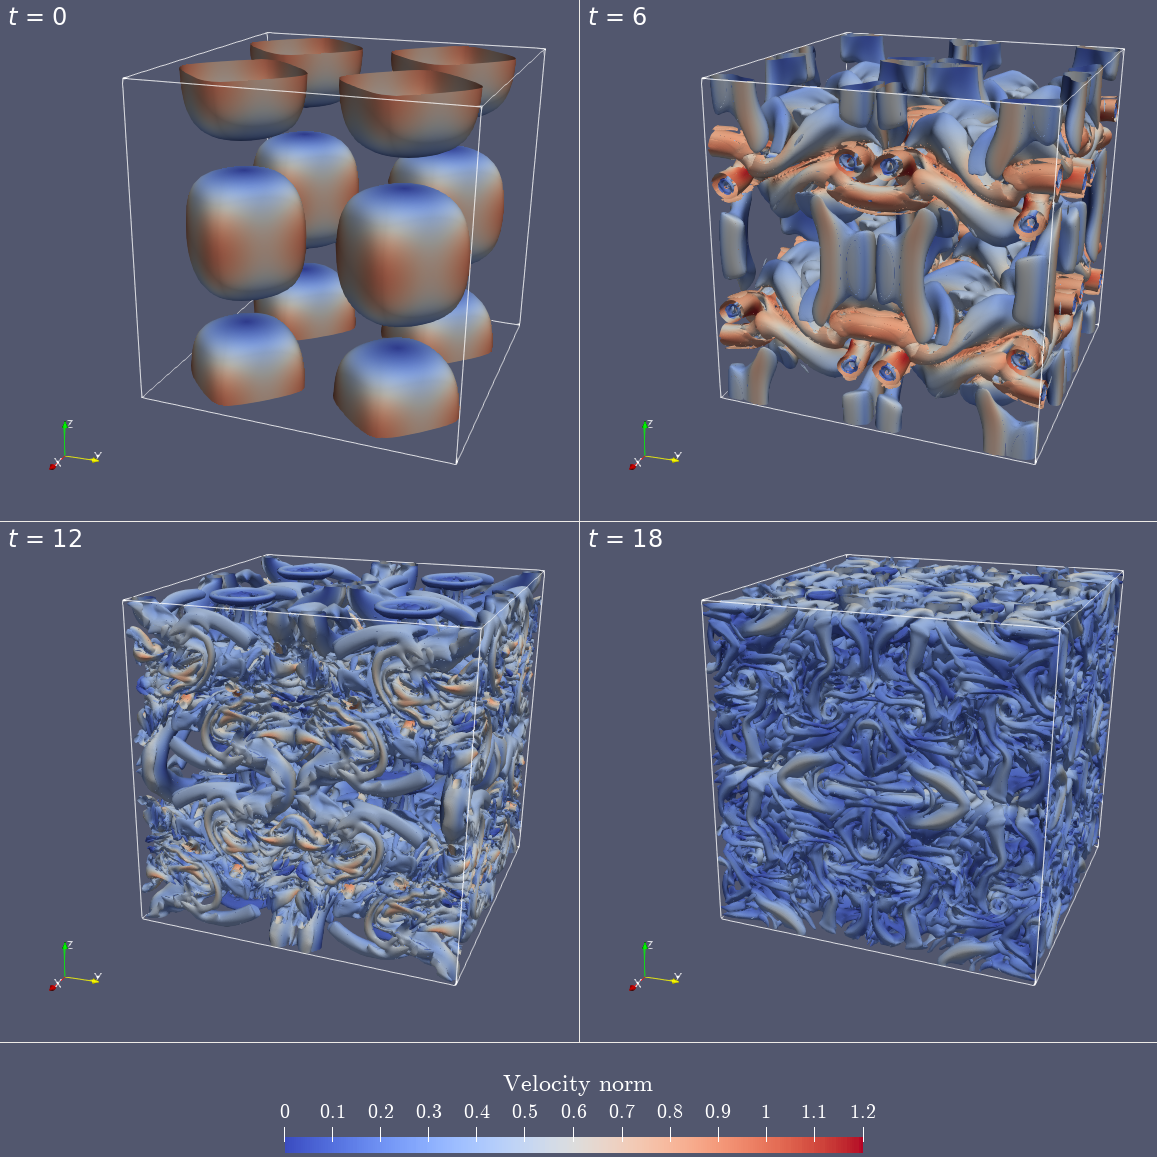
\includegraphics[width=\textwidth]{figures/tgv_fields.png}
        \caption{\PS{TODO}}
        \label{fig:tgv_fields}
      \end{figure}

      \paragraph{}
      The numerical values are non dimensionalised: $L = 1$, $\operatorname{Ma} = 0.1$, $r_\textrm{gas} = 71.4284$, $T_\infty = 1$ and $P_\infty = 71.4288$.
      The goal is to recover the Reynolds number $\operatorname{Re} = \rho_\infty U\infty L / \mu = 1600$ with the associated constant fluid viscosity is $\mu = \num{6.25e-4}$.
      The Prandtl number, ratio of momentum diffusivity to thermal diffusivity, is equal to 0.71.
      Using the convective time $t_c = L / U_\infty$, it is known that the maximum of dissipation happens around $8 t_c$, and after $15 t_c$ the flow is fully turbulent without any trace of the initial structures.
      The definition of the test case is part of the International Workshop on High-Order CFD Methods.
      A reference solution is also provided by the workshop, obtained using a spectral solver on a very refined mesh.

      \paragraph{}
      The values of interest for this test case are the temporal evolution of the mean turbulent kinetic energy over the computational domain $\Omega$:
      \begin{equation}
        E_k = \frac{1}{\rho_\infty \left|\Omega\right|} \int_\Omega \rho \frac{\norm{\vec{u}}^2}{2} \mathrm{d}\Omega ,
      \end{equation}
      the mean enstrophy, defined by
      \begin{equation}
        \mathcal{E} = \frac{1}{\rho_\infty \left|\Omega\right|} \int_\Omega \rho \frac{\norm{\nabla \times \vec{u}}^2}{2} \mathrm{d}\Omega ,
      \end{equation}
      and the kinetic energy dissipation rate, that follows the relation \PS{MAIS EN FAIT JE LA MONTRE PAS}:
      \begin{equation}
        \epsilon = -\frac{\mathrm{d} E_k}{\mathrm{d} t} = 2 \mu \mathcal{E} .
      \end{equation}
      Those values computed by the present simulation are compared with the reference values.

      \paragraph{}
      The mesh used here is the same for all computations: a regular Cartesian mesh made of $80^3$ cells.
      This choice is not natural from the workshop but previous experiments have lead to the conclusion that such a mesh gives the best solution at the lowest CPU cost, for the Spectral Difference method with the order $p = 4$.
      Each computation is run on 308 CPU cores.
      The goal is to see if the result from the simulation matches reference data up to $20 t_c$, and how much CPU time the computation took.
      The RKo6s, TVDRK(3, 3) and SSPRK(5, 4) methods are the already existing reference methods, and the exponential Rosenbrock--Euler, ExpRB32 and ExpRB42 methods are the newly implemented methods.
      For the exponential Rosenbrock methods, Krylov subspaces of dimension 20 are used for the first stage, and of dimension 5 for the additional stages for the ExpRB32 and ExpRB42 method.
      \PS{The time step is constant in a simulation, and some effort was done to use the highest time step compatible for each method.
      Above this upper bound on the time step, either the computation fails or the quality of the solution is not satisfying anymore.
      However, this higher time step can be increased for exponential methods by increasing the dimension of the Krylov subspaces used to compute $\varphi$-functions.
      By doing so, the computational cost of a single iteration is higher, but it reduces the error in the $\varphi$-functions evaluations.
      Symmetrically, it was also tried to reduce the dimension of the Krylov subspaces.
      It means that the method can not work with the same time step as before as it is now too high, but this reduces the iterations cost.
      This is to see if making more iterations that are cheaper, or in the opposite less that are more expensive can be a good idea.}
      From now on, ExpEuler($d$) method refers to the exponential Rosenbrock--Euler method that uses a Krylov subspace of dimension $d$.

      \paragraph{}
      The result of all simulation is shown in figure \ref{fig:tgv_curves}.
      As a simulation correspond to the computation with the largest time step for which the results are satisfying, this figure does not give much information: all methods produce results that are close to reference data.
      There are some differences with the reference, but all JAGUAR computations are almost undistinguishable from one another.
      As a consequence, one can argue that the error from the spatial discretisation method is the origin of the difference between
      the reference and JAGUAR computations.
      In the following, the assumption that the exact solution is provided is assumed, even if it is a numerical solution and not an algebraic one.\footnote{\PS{pas compris la phrase}}
      \PS{Apart from this error, all curves are all gathered around the same solution.}
      Indeed, we compare methods that give similar physical results, and what interests us is their statistics.

      \begin{figure}
        \centering
        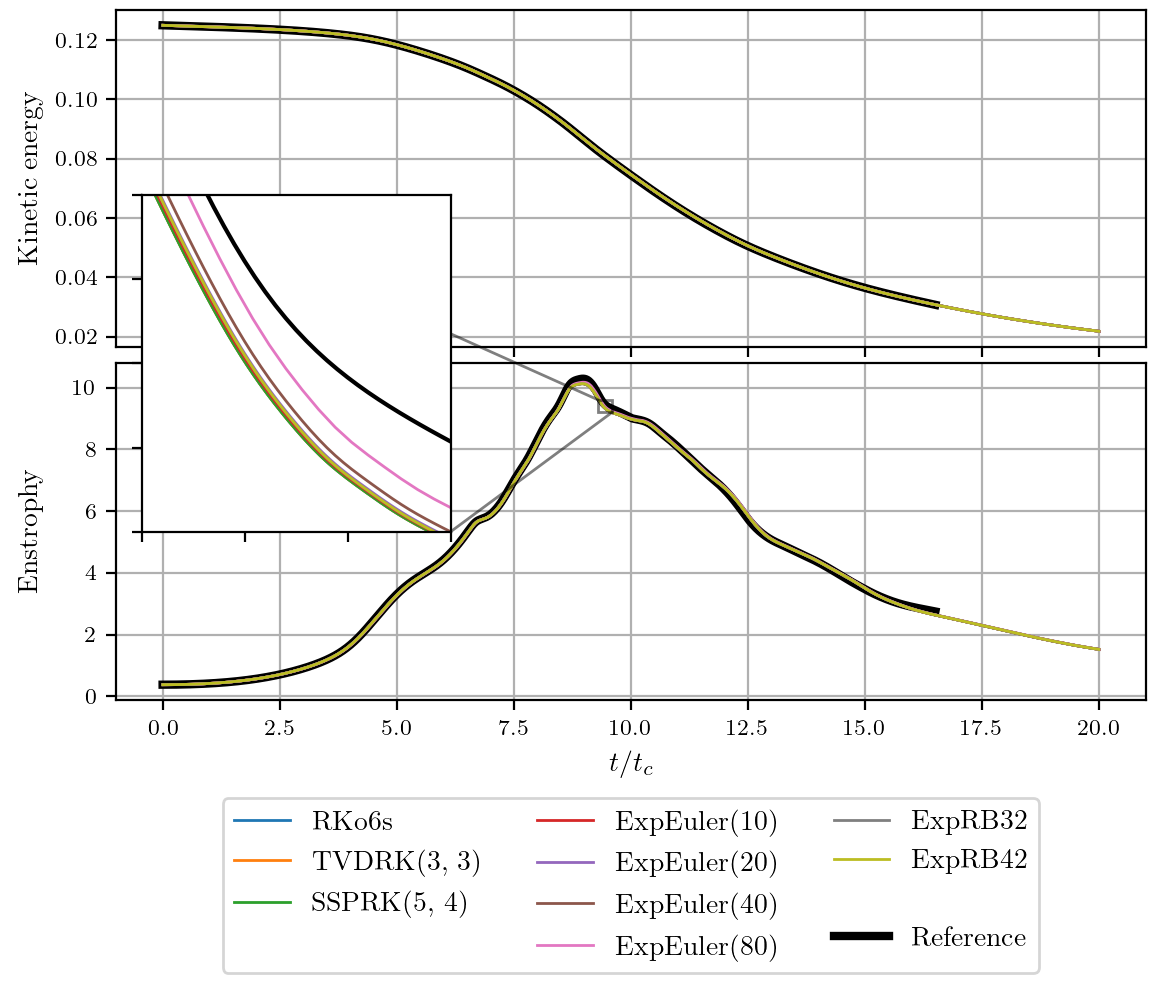
\includegraphics{figures/tgv_curves.png}
        \caption{Kinetic energy and enstrophy for various time integration methods compared to reference data.}
        \label{fig:tgv_curves}
      \end{figure}

      \begin{table}
        \center
        \begin{tabular}{c|cccc}
          Method       & $\mathcal{N}_\textrm{CFL}$ & $N_\textrm{iterations}$ & Time / iteration (s) & Total time (hh:mm:ss) \\ \hline
          RKo6s        & 0.28                       &                   50000 &                1.588 &             22:03:20  \\
          TVDRK(3, 3)  & 0.14                       &                  100000 &                0.833 &             23:08:20  \\
          SSPRK(5, 4)  & 0.28                       &                   50000 &                1.497 &             20:47:30  \\ \hline
          ExpEuler(10) & 1.4                        &                   10000 &                3.803 &             10:33:50  \\
          ExpEuler(20) & 2.8                        &                    5000 &                8.144 &             11:18:40  \\
          ExpEuler(40) & 5.6                        &                    2500 &               19.491 &             13:32:08  \\
          ExpEuler(80) & 11.2                       &                    1250 &               52.792 &             18:19:50  \\
          ExpRB32      & 2.8                        &                    5000 &               10.391 &             14:25:55  \\
          ExpRB42      & 2.8                        &                    5000 &               19.787 &             27:28:55  \\
        \end{tabular}
        \caption{
          Statistics for various time integration methods.
          Time corresponds to elapsed real time, or wall-clock time.
          A computation corresponds to the simulation of the Taylor--Green vortex from equation (\ref{eq:tgv}) on time interval $\left[0, 20 t_c\right]$.}\label{tab:tgv}
      \end{table}

      \paragraph{}
      Statistics for each time integration method are provided in table \ref{tab:tgv}.
      As the cost of the algorithms used in the time integration methods does not change between iterations, it makes sense to compute the average elapsed real time per iteration.
      Among the explicit methods, we see that the RKo6s and SSPRK(5, 4) methods run at a higher CFL number than the TVDRK(3, 3) method.
      However, they have more stages per iteration so each iteration takes longer, and the total elapsed real time is rather similar between all three methods.
      We note that the cost of one step of an explicit Runge--Kutta method is not proportional to the number of stages.
      Indeed, the implementation of the RKo6s method uses the fact that it is a low storage method to reduce the computational cost in terms of both time and memory.
      Nevertheless, the cost of an iteration of those explicit methods is much less than exponential methods.
      As expected, the cost of the exponential Rosenbrock--Euler method is similar to $d^2$ where $d$ is the dimension of the Krylov subspace used for the Arnoldi iteration \PS{vérifier ça}.
      As explained, the ExpRB32 method does not cost a lot more than the exponential Rosenbrock--Euler method that uses Krylov subspace with the same dimension.
      This is because the second stage uses only small Krylov subspace, and this is what is seen from the results in table \ref{tab:tgv}.
      We can draw two important conclusions from this analysis.
      First, we see that the exponential Rosenbrock methods are faster than the explicit Runge--Kutta methods available in JAGUAR.
      For some of them, they are almost twice as fast.
      Secondly, we see that the exponential Rosenbrock--Euler method can accurately simulate the Taylor--Green vortex at high CFL numbers.
      Accurate explicit methods would not work with such high CFL numbers, and even if implicit methods could they would not be accurate enough to capture and preserve the small scales of the flow.
      To reach high CFL numbers, we have to use larger Krylov subspaces, that make the method a lot slower.
      The method used here should not be used for actual applications: the goal was just to show feasibility.
      It seems that with exponential methods, the robustness can be increased by paying the price in terms of Krylov subspace dimension.
      We can think of ways to compute more accurately the $\varphi$-functions less expensively: by using restarted methods for instance, we can control the maximal dimension of the Krylov subspace.
      However this was not tried during this thesis.

      \paragraph{}
      This unsteady test case shows that exponential methods are interesting for our applications.
      We found a method that halves the elapsed real time, which is a great improvement for an unsteady simulation.
      We also showed that we could accurately simulate this flow while using high CFL numbers.
      It means that we have added more robust methods than the already existing ones.
      They could prove useful on applications where we are limited by the lack of stability of the explicit Runge--Kutta methods.


    \subsection{Industrial application: LS89}

      \PS{TODO}

      \paragraph{}
      We decided to try exponential methods on a last test case.
      Contrary to the previous two, we stepped out of the academic context with an industrial application.
      It is a simulation of the flow inside the LS89 turbine blade cascade that was studied experimentally by the von Karman Institute \cite{ArtsLambertdeRouvroit1992}.
      We choose this test case as it has already been done with several solvers, including JAGUAR recently \cite{BrunetCronerMinotEtAl2018}.
      We use a two-dimensional unstructured mesh, made of \num{2374} cells, that was extruded over 20 cells for a length of $0.15 c$ with $c$ the chord of the turbine blade.
      The final three-dimensional mesh made of \num{47480} cells is shown in figure \ref{fig:ls89_mesh}.
      The mesh is periodic in the extruded direction and the vertical direction.
      The boundary condition at the wall is isothermal, with $T_\textrm{wall} = 297.75 \si{\kelvin}$.
      At inlet, the stagnation conditions are $P_0 = \num{184900}\si{\pascal}$ and $T_0 = 409.2\si{\kelvin}$.
      We set the pressure at outlet at $P = \num{116487}\si{\pascal}$.


      \begin{figure}
        \centering
        % 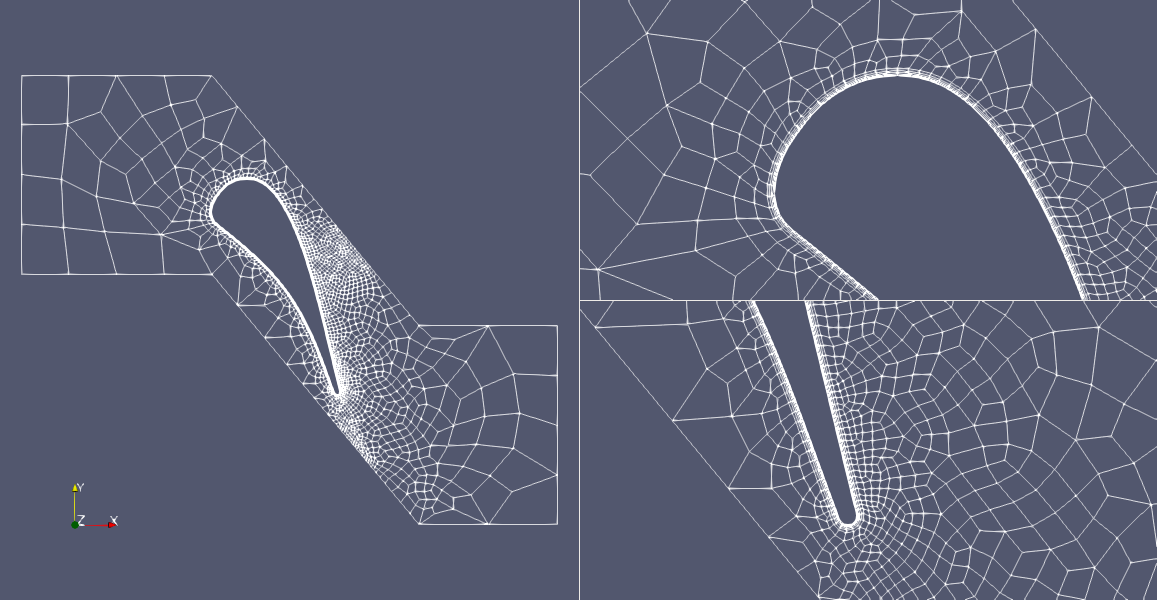
\includegraphics{figures/ls89_mesh.png}
        \caption{\PS{TODO}}
        \label{fig:ls89_mesh}
      \end{figure}
